%% The latest version of this license is in
%%   http://www.latex-project.org/lppl.txt
%% and version 1.3 or later is part of all distributions of LaTeX
%% version 2005/12/01 or later.

\documentclass{mcmthesis}
\mcmsetup{CTeX = false,   % 使用 CTeX 套装时,设置为 true
        tcn = 2301434, problem = C,
        sheet = true, titleinsheet = true, keywordsinsheet = true,
        titlepage = false, abstract = true}
\usepackage{newtxtext}
\usepackage{palatino}
\usepackage{caption}
\usepackage{subfigure}
\usepackage{pythonhighlight}

\title{Predicting Wordle Result Based on Random Forest}
%\author{\small \href{https://www.latexstudio.net/}
%  {\includegraphics[width=7cm]{mcmthesis-logo}}}
%\date{\today}


\begin{document}
\begin{abstract}
\hspace*{0.6cm} At the start of 2022, images of green and yellow squares began cropping up on Twitter, when the pandemic spreading wide on earth with people quarantined at home. It a flash in the pan and quickly gets off-booming in June which provides a good sample for Dataminer to find the regular pattern for multitude and the sociology behind.

Wordle has established itself as a popular word puzzle game by 2022. After a year, the number of Wordle players progressively decreased, and the reported data appeared to be steady. Using the dataset provided by Twitter, we were able to derive a lot of information, such as forecasting the trend of the number of people who play the game in the future and obtaining results of difficulties related to various words in word puzzles. These results will be of great significance for the company to make strategies to popularize their game.

Regarding the issue at hand in this competition, we created various models for various queries to better suit the data while yielding results. Before focusing on the need, we cleaned the data, corrected a few of its flaws, and took a quick look at its characteristics.

In problem 1(a), we applied \textbf{ARIMA (4,1,2)} model to predict the number of people who reported their results on March,1,2023, and tested it with random forest method. The \textbf{number of reported results} predicted by ARIMA is 19698. In order to further verify the reliability of our model, we applied our model to predict number in February,1,2023, results showed that the real data is also in our predicted interval, which was quite good. For problem 1(b), we use hypothesis testing, and found that there’s \textbf{no high correlation} between some basic attributes (word frequency, part-of-speech, sentiment).

In problem 2, we first created 5 factors that could affect outcomes in order to estimate the quantity of a specific term in the future: \textbf{Text\_rate, Green\_score, Yellow\_score, Combination\_score, Entropy }and employ regression using \textbf{Random Forest Regression}. Using the prediction model created in Problem 1, we replace the time parameters in this case with the number of persons. The predicted \textbf{distribution percentage} of "EERIE" is [ 0\%, 3\%, 17\%, 37\%, 32\%, 10\%, 0\% ].

In order to categorize the phrases for issue 3, we utilize \textbf{K-means} clustering and split them into 4 classes: Simple, Ordinary, Rather Difficult and Difficult. We base our standards on the means and standard deviation of test results. The word "EERIE" is categorized as \textbf{Rather Difficult} using the \textbf{Random Forest Classification}.

We attempt to recover all users' data for the final question rather than just those who contributed their answers. To do this, we create an algorithm that mimics human word guessing based on Wordle's word statistics and English word frequency, and we uncover a wealth of intriguing data by taking into account players who tweet their game results.

\begin{keywords}
Wordle, ARIMA, Hypothesis-testing, Random Forest, Entropy, K-means
\end{keywords}
\end{abstract}
\maketitle

%% Generate the Table of Contents, if it's needed.
\begin{spacing}
\tableofcontents 
\end{spacing}
\newpage
%%
%% Generate the Memorandum, if it's needed.
%\memoto{\LaTeX{}studio}
%\memofrom{Liam Huang}
%\memosubject{Happy \TeX{}ing!}
%\memodate{\today}
%\logo{\LARGE I'm pretending to be a LOGO!}
%\begin{memo}[Memorandum]
 %\lipsum[1-3]
%\end{memo}
%%

%%%%%%%%%%%%%%%%%%%%%%%%%%%%%%%%%%%%%%%%%%%%%%%%%%%%%%%%%%%%%%%%%%%%%

\section{Introduction}
\subsection{Problem Background}

\hspace*{0.6cm} Wordle has become a cultural phenomenon, with players all over the world competing to get the highest scores and share their strategies and tips for success. The game has also sparked debate and discussion around issues such as the ethics of using external tools to cheat and the impact of the game on mental health and productivity.

\subsection{Literal Review}

\hspace*{0.6cm}Morning Consult, a global data intelligence company, found that Wordle was one of the top ten most popular mobile games in the United States in January 2022, with an estimated 9.6 million monthly active users.[1]

However, it's important to note that these surveys were conducted early in the game's rise to popularity and may not reflect the current level of interest or engagement with the game. As Wordle is a relatively new phenomenon, there is likely to be more data and surveys on the topic in the future.

Another survey conducted by OnePoll in January 2022 found that nearly three-quarters of respondents (73\%) had played Wordle at least once, and of those who had played the game, 40\% reported playing it every day.[3]

Through utilization of the extant survey, we were afforded a panoramic view of its ubiquity, culminating in a refined, precise, and attainable blueprint for our architectural design.
\subsection{Our Work}
\hspace*{0.6cm}After processing the data to a more accurate version, we do a prediction of number of people sharing on Twitter in the upcoming few days. It is the Variation towards time model. Furthermore, we discover a connection between Word Attributes and peoples' specific casting preferences in the hard mode. In the fifth section, we forecast how individuals would do given a specific phrase and predefined time. We created a Classify Words Model after extensively learning from existing models. It can give a profit of a word from the result side.

What's more intriguing is that, in contrast to the surveys mentioned above, we focused on the interesting features of this game, from which we created new neural network learning algorithms to abstract "a changing throng" and analog the distribution of the actual number of players when playing this game, regardless of whether they tweeted their results or not. There after, We discovered a correlation between the frequency with which people solve this challenge and their desire to share it on Twitter from the Analog Gamer Mass, which is in line with psychological studies.

%%%%%%%%%%%%%%%%%%%%%%%%%%%%%%%%%%%%%%%%%%%%%%%%%%%%%%%%%%%%%%%

\section{Preparation of the Models}
\subsection{Data Processing}

\hspace*{0.6cm}After examing the provided excel, we pictured the properties and found noises inside.There are four words "na$\ddot{i}$ve","tash","clen","rprobe" appeared invalid during the String Matching Process. According to the daily use practice and later model, we change them to "naive", "trash", "clean" and "probe" respectively. 

To make the supplied Attempt-partition more practicable, we use 3 Sigma Outlier Identification and found the sum of all ratios happened to be far away from the rational value 1.
\[ \Sigma_{i=1}^{7}t_i = 1.26 \] 
Owing to this spot, we manipulated \[ t_i' = 1/1.26 * t_i \]
to acquire \[ \Sigma_{i=1}^{7}t_i' = 1 \] 
which fits the general knowledge and the topic requirements. 

\hypertarget{notation}{%
\subsection{Notation}\label{notation}}

\begin{longtable}[]{@{}20@{}}
\toprule\noalign{}
Symbol & Definition \\
\midrule\noalign{}
\endhead
\bottomrule\noalign{}
\endlastfoot
\(EN\) & Entropy \\
\(TR\) & Text\_rate \\
\(GS\) & Green\_score \\
\(YS\) & Yellow\_score \\
\(CS\) & Conbine\_score \\
\(\mu\) & Mean Value \\
\(\sigma\) & Standard Deviation \\
\(Skew\) & Skewness \\
\(Kurt\) & Kurtisis \\
\end{longtable}

\subsection{Overall Flowchart}

\begin{figure}[h]
\small
\centering
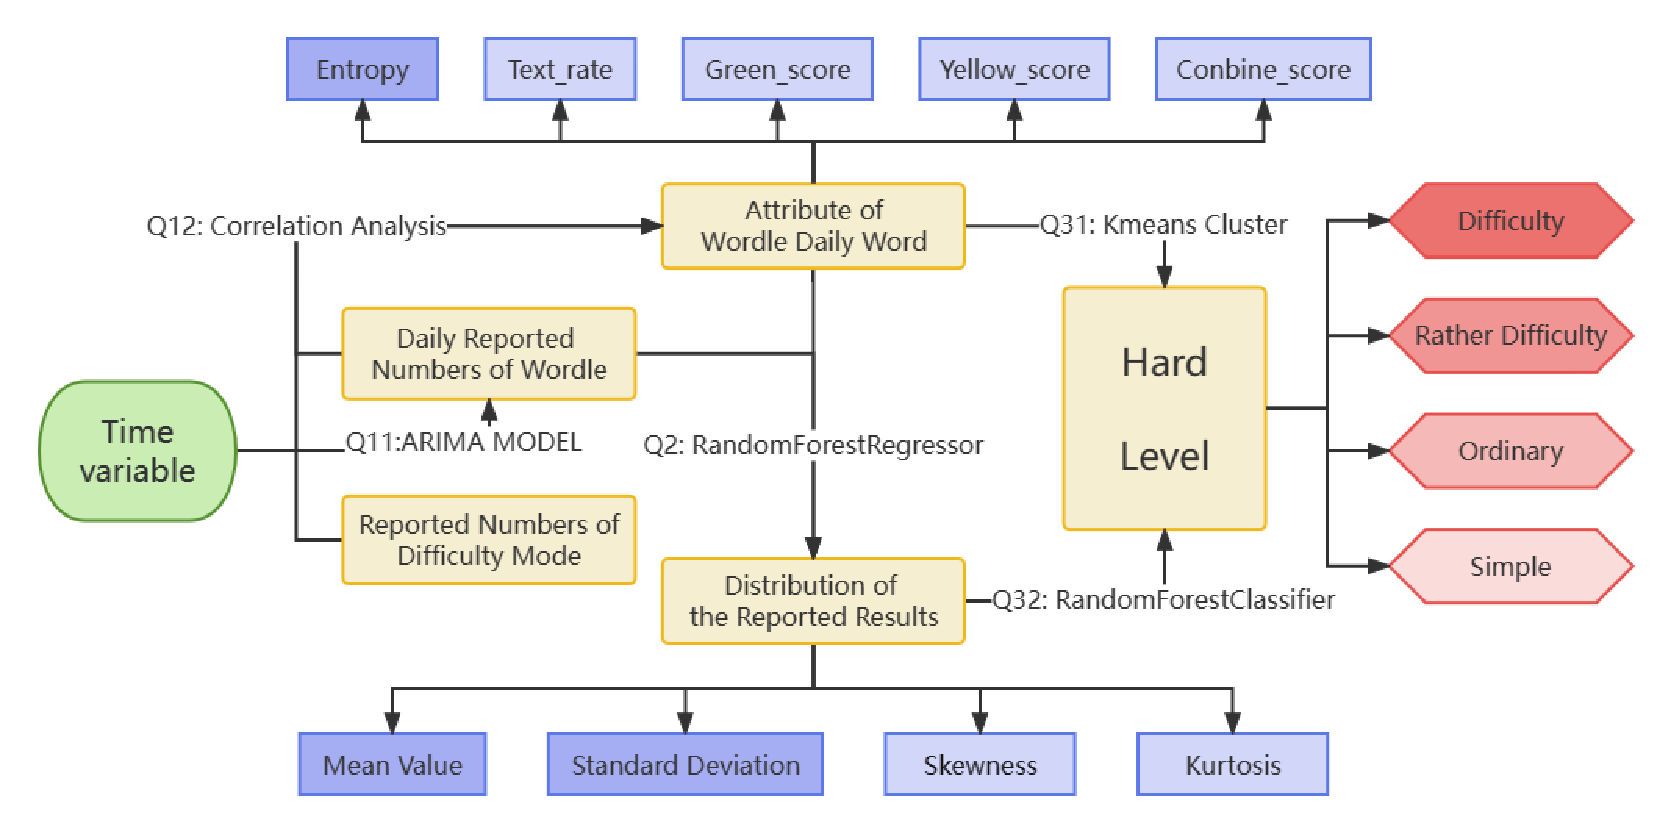
\includegraphics[width=13cm]{overall}
\caption{Overall Flowchart} \label{fig:aa}
\end{figure}


%%%%%%%%%%%%%%%%%%%%%%%%%%%%%%%%%%%%%%%%%%%%%%%%%%%%%%%%%%%%%%%3

\section{Variation towards time model }
\subsection{Problem Analysis}
\subsubsection{Problem Restatement}

\hspace*{0.6cm}According to the subject, we clarify the requirement to two parts.
\begin{itemize}
\item Develop the model to explain the variation (Regression Fitting) 
\item Use the model for predictive analysis (Forecasting) 
\end{itemize}

The first problem is mainly a Time Series Analysis issue. Thereafter preprocessing the data, we found the outliers and corrected the data by approximate mean. Here is the Time Series Plot of the Original Data and a Time Series Plot of the First-order Difference Data.
\begin{figure}[htbp]
\centering    %居中
\subfigure[Time-series Diagram of First-order differencing] %第一张子图
{\begin{minipage}{8cm}
\centering          %子图居中
\includegraphics[scale=0.5]{0time_series}   %以pic.jpg的0.5倍大小输出
\end{minipage}
}	
\subfigure [Time-series Diagram of Zero-order differencing] %第二张子图
{\begin{minipage}{8cm}
\centering      %子图居中
\includegraphics[scale=0.5]{1time_series}   %以pic.jpg的0.5倍大小输出
\end{minipage}
}
\caption{name of the figure} %  %大图名称
\label{fig:1}  %图片引用标记
\end{figure}

Since this data has no obvious periodic characteristics, there is no periodicity in the amount of data for one year. Observing that the first-order difference plot predicts the first-order difference is a smooth data, we are ready to use the traditional ARIMA model for interpretation and prediction. In order to verify the suitability of the model, we also adopt the Desicion Tree Regressor model for comparison prediction.

\subsubsection{Flowchart}

\begin{figure}[h]
\small
\centering
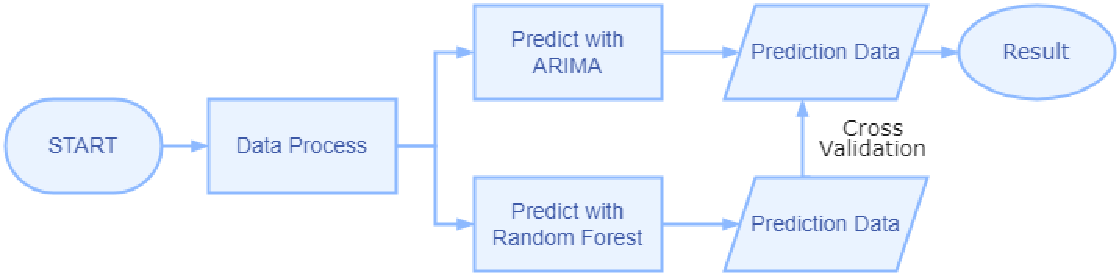
\includegraphics[width=10cm]{Q11}
\caption{Flow Chart} \label{fig:aa}
\end{figure}

\subsection{Model Construction}

\subsubsection{Model Principle}

\hspace*{0.6cm}ARIMA model is a Time Series Prediction Model which can be used to forecast future time series trends. ARIMA has three terms that correspond to the three main components of the model, respectively stands for self-regression (AR), difference (I) and moving average (MA). Autoregressive (AR) refers to the use of past observations to predict future observations. The model assumes that future values are a linear combination, where the weights are controlled by the autoregressive coefficients (AR coefficients). Moving average (MA) refers to the use of past forecast errors to predict future observations. The model assumes that the future values are a linear combination of past forecast errors, where the weights are controlled by the moving average coefficients (MA coefficients). The weights are controlled by the moving average coefficients (MA coefficients). Differencing (I) refers to the differencing of the time series to make it smooth (i.e. mean and variance do not change over time). 

By differencing the time series one or more times, the ARIMA model can remove the trend and seasonality, thus making the time series smooth. A smooth time series can be more easily modeled and predicted. 

A regression tree is a decision tree based machine learning algorithm for regression analysis of continuous data. The basic idea of regression tree is to recursively divide a data set into regions, each region is represented by a constant that represents the output values of all data points within that region. The regression tree recursively divides the dataset into regions until only one data point remains in each region or a predefined stopping condition is reached.

The general formula we use for ARIMA(p, d, q) model can be written as:

\[y_t = c + \phi_1y_t-1 + ... + \phi_py_t-p + \theta_1e_t-1 + ... + \theta_qe_t-q + e_t\]

where, $y_t$ is the value of the time series at time t
,$c$ is a constant (or intercept term), $\phi_1,...,\phi_p $ are the autoregressive coefficients of lag 1 through p,
$\theta_1,...,\theta_q$ are the moving average coefficients of lag 1 through q,
$e_t$ is the error (or residual) term at time t, which is assumed to be normally distributed with mean zero and constant variance,
d is the order of differencing required to make the time series stationary.


The autoregressive component of the model (AR) captures the dependence of the current value on the previous p values of the time series. The moving average component (MA) captures the dependence of the current value on the past q error terms. The order of differencing (d) determines the number of differences required to make the time series stationary, which is a necessary condition for an ARIMA model.

The parameters ($\phi_1, ..., \phi_p, \theta_1, ..., \theta_q$) are estimated from the data using various methods, such as maximum likelihood estimation or least squares estimation. Once the parameters are estimated, the model can be used for forecasting future values of the time series.

\subsubsection{Model Assumption}

\hspace*{0.6cm} 1. the number of daily reports is only time-dependent, i.e., the difficulty coefficient of the word of the day, the number of people who chose the difficult mode and the percentage of the number of attempts and other indicators not mentioned are not relevant for the number of daily reports.

2. the first-order difference of the data is divided into a smooth time series

3. Only the data from January 7, 2022 to December 31, 2022 are known to make the prediction, without considering the influence of chance factors such as the increase of game attention due to the American game on the game's enthusiasm.

\subsubsection{Main Model}

\hspace*{0.6cm}1. Testing the smoothness of first-order difference time series with ADF unit root.

\begin{table}[!htbp]
\begin{center}
\caption{Test Outcome}
\begin{tabular}{cl}
	\toprule
	\multicolumn{1}{m{3cm}}{\centering Parameter}
	&\multicolumn{1}{m{4cm}}{\centering Value}\\
	\midrule
	ADF & -7.1359413592169885\\
	p &3.4210335686568374e-10\\
	1\%Confident Value &-3.4496162602188187\\
	\bottomrule
\end{tabular}\label{tb:notation}
\end{center}
\end{table}
There is greater than 99\% probability of rejecting the original hypothesis, so the series is a smooth time series.

2. Ljung-Box test is used to verify whether the series is white noise

Each p-value is less than 0.05 or equal to 0, which means that the data is not white noise data and the data is valuable to continue the analysis.

3. Draw pacf plot and acf plot\begin{figure}[htbp]
\centering    %居中
\subfigure[PACF] %第一张子图
{\begin{minipage}{8cm}
\centering          %子图居中
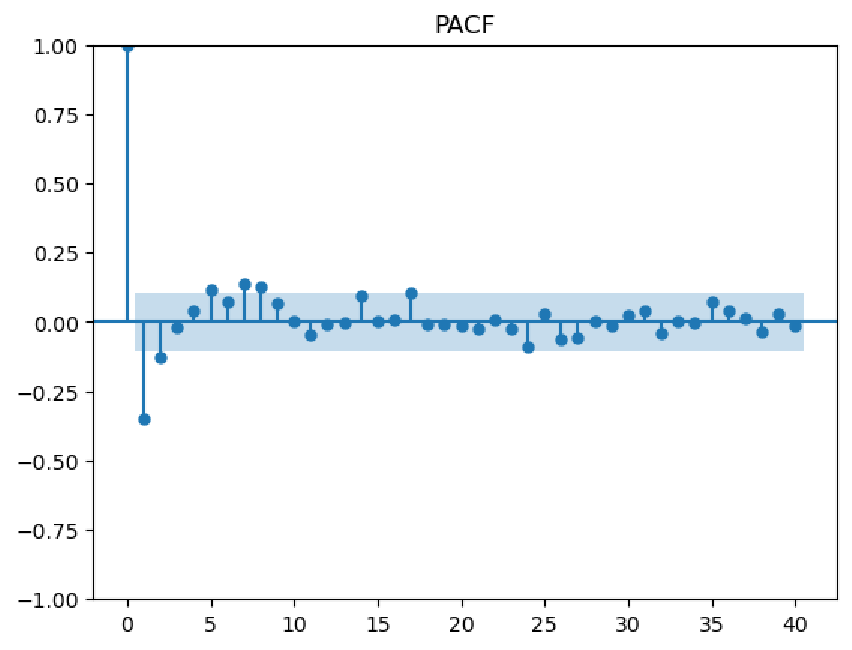
\includegraphics[scale=0.5]{PACF}   %以pic.jpg的0.5倍大小输出
\end{minipage}
}	
\subfigure [ACF] %第二张子图
{\begin{minipage}{8cm}
\centering      %子图居中
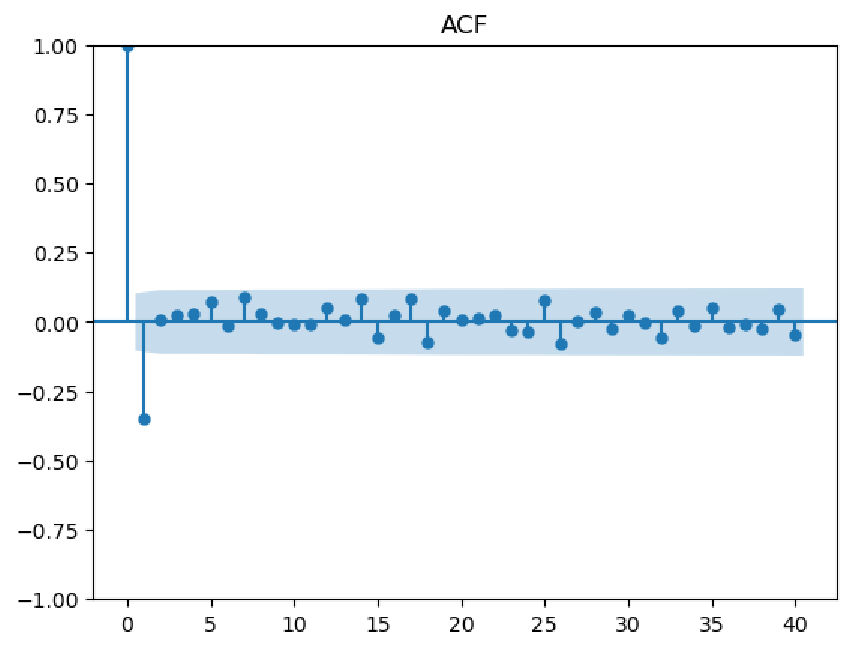
\includegraphics[scale=0.5]{ACF}   %以pic.jpg的0.5倍大小输出
\end{minipage}
}
\caption{ACF and PACF} %  %大图名称
\label{fig:1}  %图片引用标记
\end{figure}

4. Model tuning

Determination of AR() and MA() model parameters by heat map\begin{figure}[h]
\small
\centering
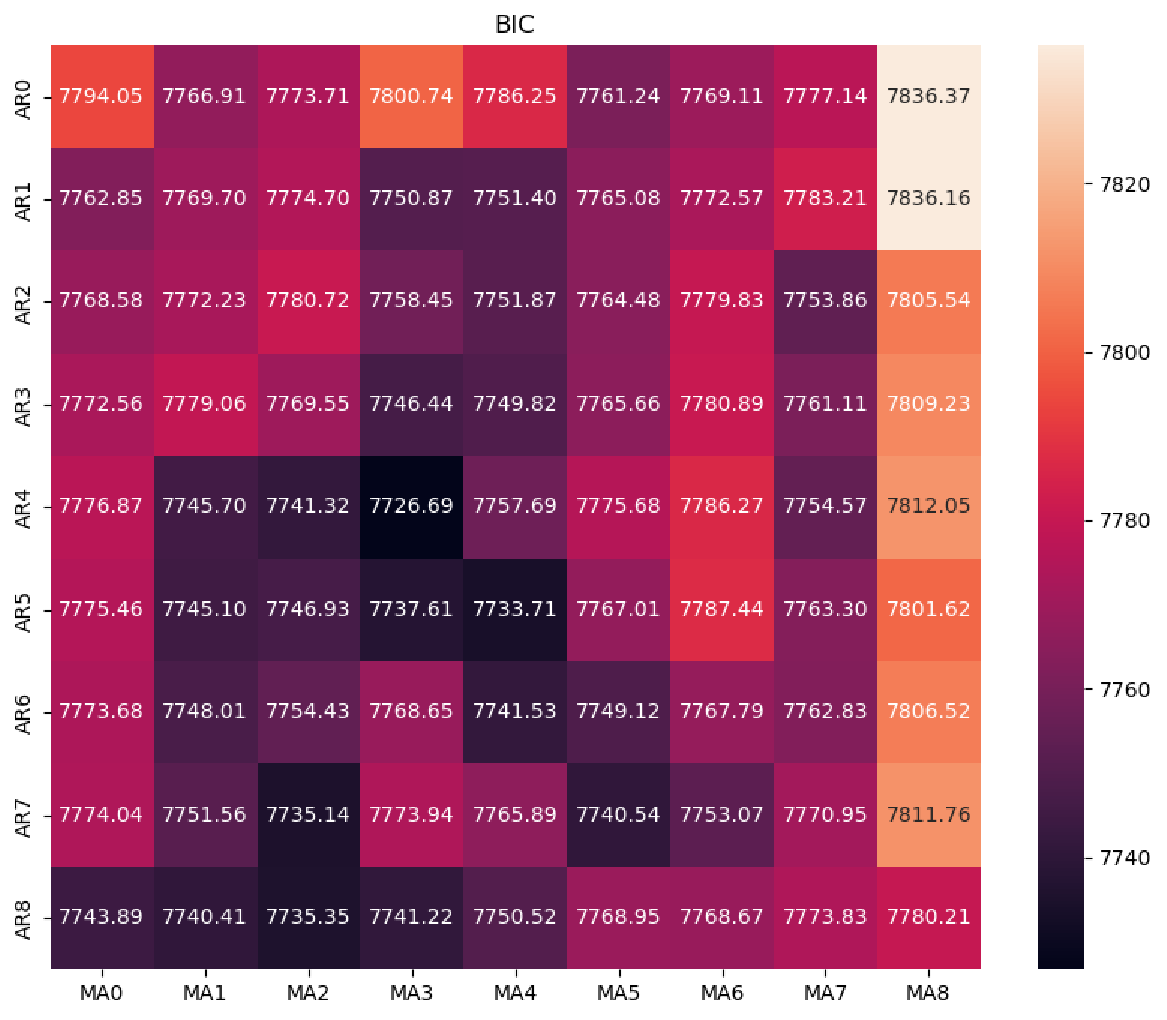
\includegraphics[width=7cm]{thermodynamic}
\caption{Thermodynamic Graph} \label{fig:aa}
\end{figure}

5. With comprehensive consideration, we made a decision to fit the ARIMA(4,1,2) model to the time series, where we found the ultimate answer for our prediction.

\[\left(1-\sum_{i=1}^4 \alpha_i L^i\right)(1-L)^1y_t=\alpha_0+\left(1+\sum_{i=1}^2 \beta_i L^i\right) \varepsilon_t \]

In order to preclude the deviation caused by the conventional model, we put up the Random Forest Method for further validation.

\begin{figure}[htbp]
\centering    %居中
\subfigure[ARIMA(4,1,2)] %第一张子图
{\begin{minipage}{8cm}
\centering          %子图居中
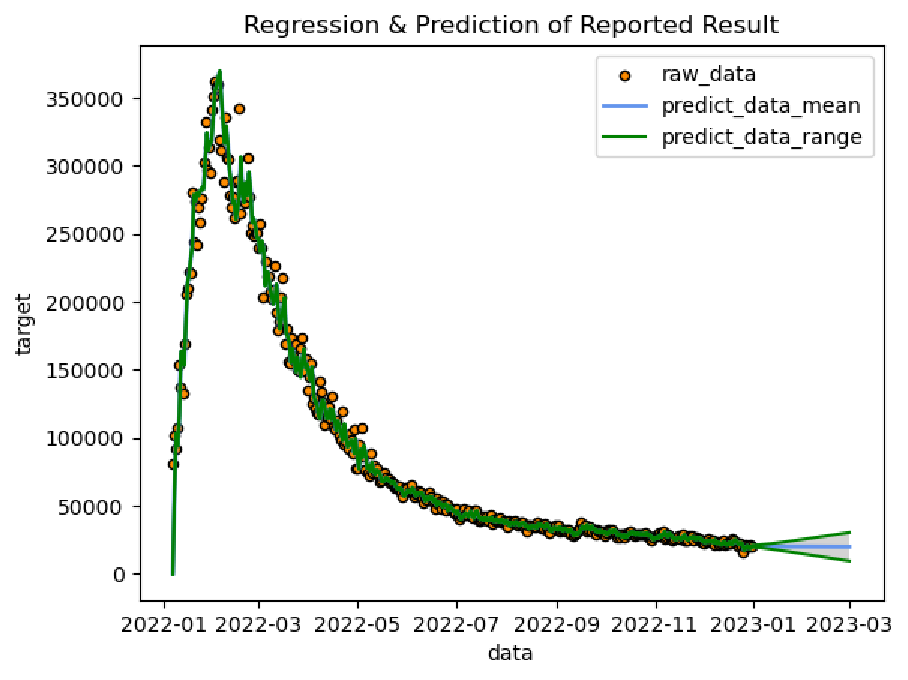
\includegraphics[scale=0.5]{predict}   %以pic.jpg的0.5倍大小输出
\end{minipage}
}	
\subfigure [Regression Tree] %第二张子图
{\begin{minipage}{8cm}
\centering      %子图居中
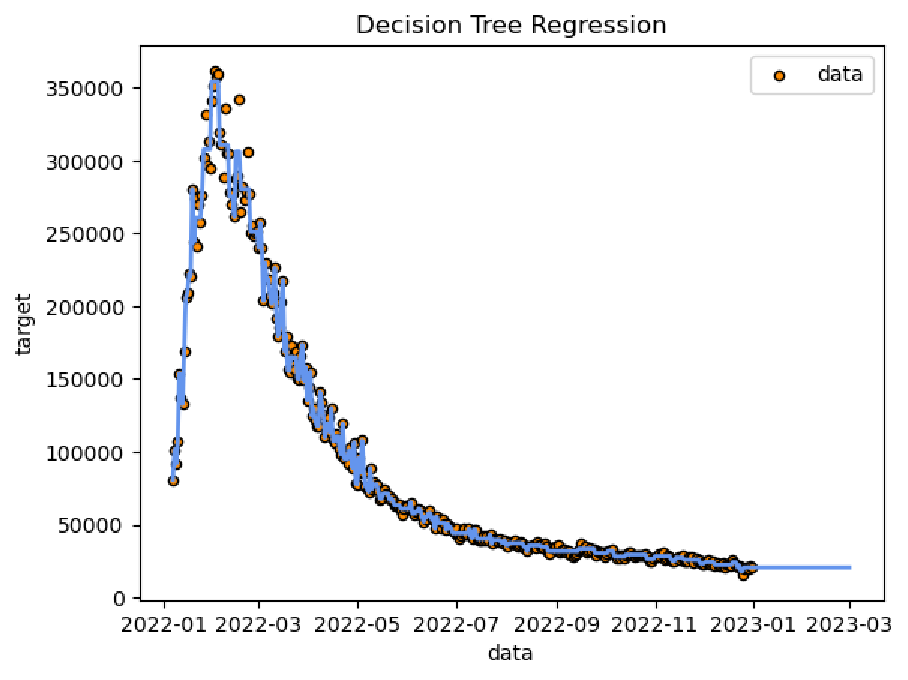
\includegraphics[scale=0.5]{regression_tree}   %以pic.jpg的0.5倍大小输出
\end{minipage}
}
\caption{Predicts} %  %大图名称
\label{fig:1}  %图片引用标记
\end{figure}


\subsection{Result} 
\subsubsection{Specifically on March 1, 2023}
\hspace*{0.6cm}From the ARIMA model, we figure out the prediction interval for the number of reported results on March 1, 2023
\begin{itemize}
\item The mean of the prediction interval is: 19697.53 = 19698
\item Upper limit of the prediction interval: 30148.69 = 30149
\item Lower limit of the prediction interval: 9246.36 = 9246
\end{itemize}


\subsubsection{Random forest method}
\hspace*{0.6cm}This is for further validation with a training accuracy of 0.98259.

Predicted value: 20439.16 = 20439.

\subsection{Sensitivity Analysis }
\hspace*{0.6cm}From the ARIMA model, we can predicte the number of reports on a "future time" such as Feburary 1th.
\begin{itemize}
\item The mean of the prediction interval is: 19847.08 = 19847
\item Upper limit of the prediction interval: 25321.29 = 25321
\item Lower limit of the prediction interval: 14372.87 = 14373
\end{itemize}

\begin{figure}[h]
\small
\centering
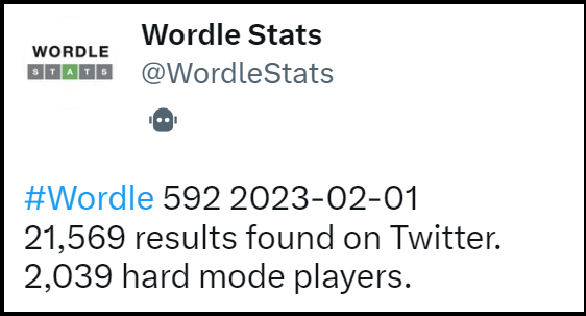
\includegraphics[width=7cm]{twitter}
\caption{Data From Twitter[2]} \label{fig:aa}
\end{figure}
The realistic result basically lies in the center of the prediction interval, which proves that the model fits well. The sensitive stability can be strengthened by the two different prediction models.


%%%%%%%%%%%%%%%%%%%%%%%%%%%%%%%%%%%%%%%%%%%%%%%%%%%%%%%%%%%%%%%333333333

\section{Influence of Word Attributes on Hard Choices}
\subsection{Problem Analysis}

\hspace*{0.6cm}In this section, we aim to figure out whether there are attributes of the word that affect the percentage of scores reported that were played in Hard Mode.
 
Attributes means the characteristics or properties that can be used to describe or define a word. Some common word attributes include part of speech, synonyms, antonyms, definition, pronunciation, etymology, and usage. [4] After condensing this classification, we focus on three basic attributes: Appearance Rate ( AR), Sentiment Value (SV) and the part of speech (POS).

Here is the chart for better comprehension of what we did on this problem.

\begin{figure}[h]
\small
\centering
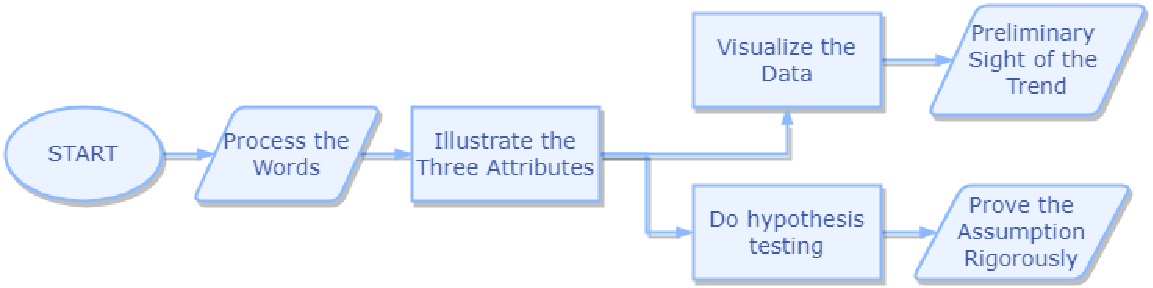
\includegraphics[width=10cm]{Q12}
\caption{Flow Chart} \label{fig:aa}
\end{figure}

\subsection{Model Construction}
\subsubsection{Model Assumption}
\hspace*{0.6cm}We introduce three character for you in this section as three main attributes of a word. 

They are:
\begin{itemize}
\item The first one describe the rate one letter happens to show up at a certain slot with the support of all words in corpus, the complete potential word set. We name it Appearance Rate (AR). 
\item Every word has its sentiment value(SV) in the human view. Some negative like "bitter", some positive as "happy" and some with even affections like simple object nouns. We quantify this emotion and take it into consideration to see whether it can effect the frequency people choose the hard mode.
\item Part of speech (POS) is the characteristic or property of a certain word, crudely be divided into Verbs, Nouns, Numerals, Adjectives, Adverbs, Pronouns, Articles, Prepositions, Conjunctions, Interjections and so on.
\end{itemize}

\subsubsection{Main Model}

\hspace*{0.6cm}We mainly use wolftram’s word frequency data to get the frequency words in Wordle, and use python NKTL tool to analyze word’s sentiments and POS.

Firstly, we draw 3 pictures to reflect the correlation between sentiment, word frequency, and pos directly. Since there’re many words with POS that are less than 10 word in word set (359), thus we drop these data out in order to increase the robustness of our model

Among the multiple data obtained by classification, most types of words have outcome data below To improve the robustness and reliability of the data, we selected data sets which has a value above 10 for concentration, including nouns (NN) adjectives (JJ) verbs (VB).


\begin{figure}[h]
\small
\centering
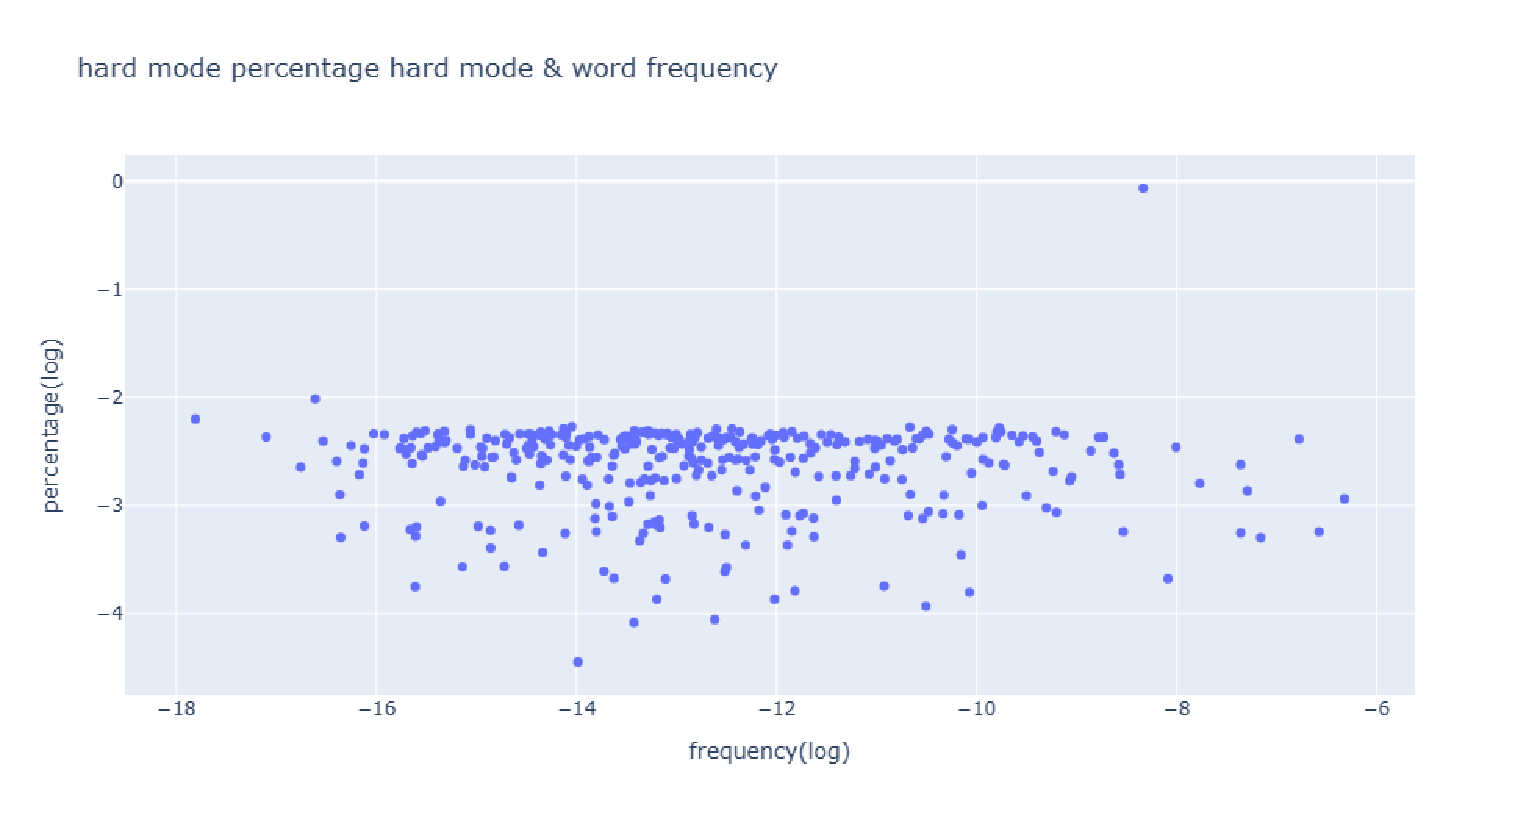
\includegraphics[width=10cm]{222}
\caption{} \label{fig:aa}
\end{figure}

Seen for the data, we assume that these data do not have a strong correlation with each other, In order to test our assumption, we did Pearson correlation coefficient analysis and hypothesis testing. 

\subsection{Result}
\hspace*{0.6cm}The results of POS are [NN: 079, JJ: 0.075, RB: 0.079909, VBP: 0.079609, VBD: 0.082291],which leads to irrelevant relationship between the two perspectives.

Pearson hypothesis testing( Two-sided Hypotheses ):  

\hspace*{3cm}sig - corrrelation

\hspace*{1.2cm}sentiment: 0.395 - 0.045 

\hspace*{1.2cm}frequency: 0.89 - 0.007

Since all the correlation are small (absolute value<0.1) and p value in hypothesis testing’s absolute value are much greater than 0.05, thus we’re 95\% sure the correlation between them is not significant, so the assumption holds.



%%%%%%%%%%%%%%%%%%%%%%%%%%%%%%%%%%%%%%%%%%%%%%%%%%%%%%%%%%%%%%%44444444444

\section{Predict the Distribution}
\subsection{Problem Analysis}

\begin{itemize}
\item Development of the model for future dates future scenario words and reported its results. Gives percentages of (1, 2, 3, 4, 5, 6, X) for "EERIE" on March 1, 2023
\item uncertainty of the model prediction 
\item the confidence of the model prediction 
\end{itemize}

\subsection{Model Construction}

\subsubsection{Model Principle}
\hspace*{0.6cm}Random Forest Model can handle very high dimensional data and does not have to do feature selection (because the feature subset is chosen randomly), so for our multiple features, the random forest model works well. And to better observe the uncertainty, random forest can give which features are more important, and changing important features is more likely to perturb the model to determine the sensitivity and uncertainty of the model.

\subsubsection{Model Assumption}

\hspace*{0.6cm}1. it is assumed that the time parameter only affects the number of reports per day, independent of the difficulty of the questions, the quality of the participants and the accumulated game experience. 

2. The standard deviation of the report distribution is assumed to be independent of the kurtosis and word properties. 

3. It is assumed that the noise caused by chance does not mask the characteristics of the mean and skewness

\subsubsection{The Four New Variants}

\hspace*{0.6cm}This is the second question mapping to the requirement we dig more data attributes 

1. \textbf{The combine\_score} 

When two word appears to be a combination in a word, people are prone to choose the one their more familiar with. It is known as the "preferred-candidate effect" or "lexical bias," which refers to the tendency of people to select the more familiar word when encountering a combination of two words. Once a study found that the familiarity of the constituent words affected the processing of compounds in the brain, with more familiar words being processed faster.[6]

Due to the five-word limit, we only extract the two-word combination in English Letter Frequency. With data found in \url{http://norvig.com/mayzner.html}, we score each of the words by identity the two words combination inside them.

For example, we got the word "intro". Put it into the word pool, we have "in" stands for possibility of 2.43,  "ro" stands for possibility of 0.73, "nt" stands for possibility of 1.04, finally the sum reaches 4.30, which is the value of  the  combine\_score  of  "intro".

2. \textbf{The green\_score}

Follow the principal of the game, when a letter reaches it right position in a word, Wordle will appear green in the corresponding place. It gives a good perspective to identify the importance of a word, so that we decided to score a word by the possibility it appears correct on its position. An important attribute for a word is the way it arranged. And the position it occupied has its possibility influence on the possibility we guess right. Here is the way we design to quantify this characteristic.

As far as we've concerned, the overall letter may be shown on Wordle is 2315, which is selected by creator Wordle in the 12972 valid words [5]. 

For every letter in this database, we denote it as $a_{i}$ and divide it into five parts by site. $a = [x_{11},x_{12},x_{13},x_{14},x_{15}]$

Here is the notation for the subsequent algorithm.

\[Letter\_score(x_{ij})=\frac{the\ total\ appearance\ time\ of\ x_{ij}\ on\ position\ j}{ the\ total\ appearance\ time\ of\ all\ letter\ on\ position\ j } \]

\[ Word\_score(a_i)=Σ(1-5) x_{ij}* Letter\_score(x_{ij}) \]


3. \textbf{The yellow\_score}

The target of yellow score is with similarity to green score, which will measure the possibility of how many in a certain word will turn yellow if put into the game’s chart.
 We define a Letter’s score and word’s yellow score as follows:

\[Letter_score(x_ij) = \frac{the\ total\ appearance\ time\ of\ this\ letter\ in\ \all position}{the\ total\ appearance\ time\ of\ all\ letter\ in\ all\ position }
\]

\[ Word_score = Σ(1~5) {x_{ij}* Letter_score(x_ij)} \]
 
4. \textbf{Entropy}

The more we know about Wordle, the more "information" we want to get with each guessing attempt. In other words, if I eliminate more words in a single attempt, the more likely we are to win the Wordle game with fewer attempts.

An intuitive conclusion in information theory is that the more information we have about a situation, the less likely we are to encounter it. So how do we measure the expectation that a word will give us information? Information entropy helps us explain the relative amount of information that a word can give us.

The formula of information entropy is defined as follows:
\[ EN=-\sum_{i=1}^n P\left(x_i\right) \log p\left(x_i\right)\]

Where $P$ is defined as the probability of a certain color combination, and $p$ is defined as the proportion of the number of words left by the information provided to the total words

We found that at the first guess, the information entropy of each word was the same regardless of the answer to the riddle, which can be used as an indicator to measure the properties of a word. Here's the code to compute the entropy of information:

\begin{python}
for every input x
	go through the database for 243 cases
	score x with Wordle rules
	if reaches grey
		add 0 mark
	else if reaches yellow
		add 1 mark 
	else add 2 marks
	obtain P = vertex[p1,p2,...p\_2315]

	then find the appearance rate for each corlor composition in the database
	f = vertex[f1,f2,...,f\_2315]
	put the P and f as p and P in the previous formula
\end{python}

And we found that the distribution of the data set given by the question, i.e., the correlation percentage of future dates (1,2,3,4,5,6,X), is a fixed order data, all have some correlation, so we use the method of plotting histograms and fitting the data.

The correlation percentages are interpreted as the mean, standard deviation, skewness, and kurtosis. The approximate distribution of these four values is as follows

\begin{figure}[htbp]
\centering    %居中
\subfigure[] %第一张子图
{\begin{minipage}{3.3cm}
\centering          %子图居中
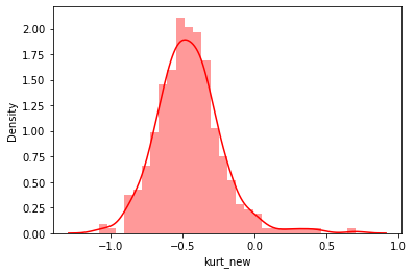
\includegraphics[scale=0.5]{1}   %以pic.jpg的0.5倍大小输出
\end{minipage}
}	
\subfigure [] %第二张子图
{\begin{minipage}{3.3cm}
\centering      %子图居中
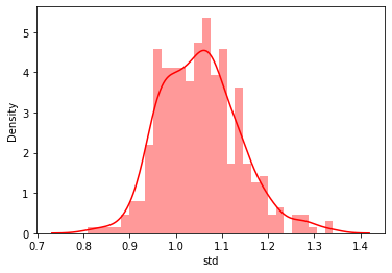
\includegraphics[scale=0.5]{2}   %以pic.jpg的0.5倍大小输出
\end{minipage}
}
\subfigure[] %第一张子图
{\begin{minipage}{3.3cm}
\centering          %子图居中
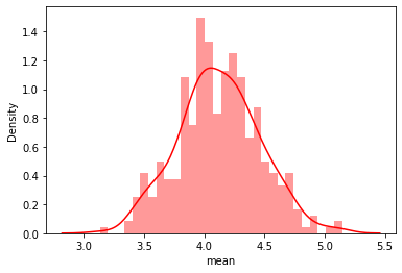
\includegraphics[scale=0.5]{3}   %以pic.jpg的0.5倍大小输出
\end{minipage}
}
\subfigure[] %第一张子图
{\begin{minipage}{3.3cm}
\centering          %子图居中
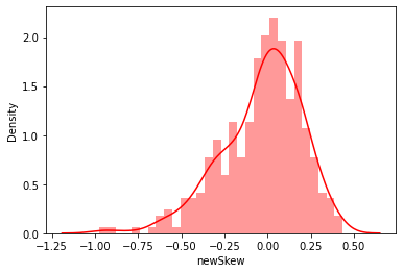
\includegraphics[scale=0.5]{4}   %以pic.jpg的0.5倍大小输出
\end{minipage}
}
\caption{Predicts} %  %大图名称
\label{fig:1}  %图片引用标记
\end{figure}

Through correlation analysis, we found that skewness and kurtosis are basically uncorrelated with word attributes, and the mean and standard deviation correlations are low enough to be analyzed as two independent indicators.

For the consideration of the time direction, since we used the ARIMA model in the first question to give the relationship between time and the number of reporters, in this question, we used the number of reporters instead of time to influence the distribution of the reported results. Thus, by regressing the random forest regression model, we use the five dimensions of the indicators to map the mean and standard deviation of the two indicators, and fit the mean and standard deviation to the distribution function.
  

\begin{figure}[htbp]
\centering    %居中
\subfigure[Mean] %第一张子图
{\begin{minipage}{8cm}
\centering          %子图居中
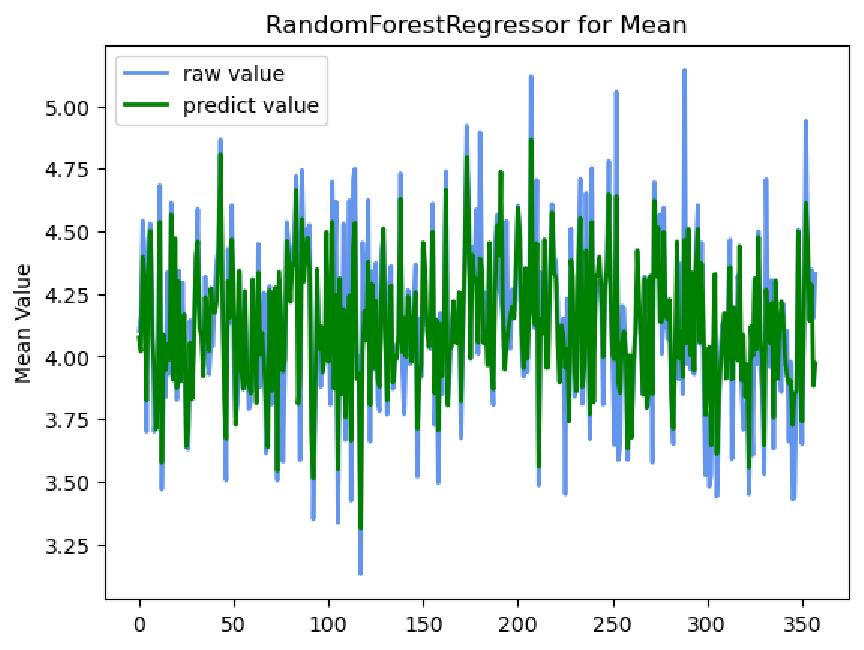
\includegraphics[scale=0.5]{x}   %以pic.jpg的0.5倍大小输出
\end{minipage}
}	
\subfigure [Var] %第二张子图
{\begin{minipage}{8cm}
\centering      %子图居中
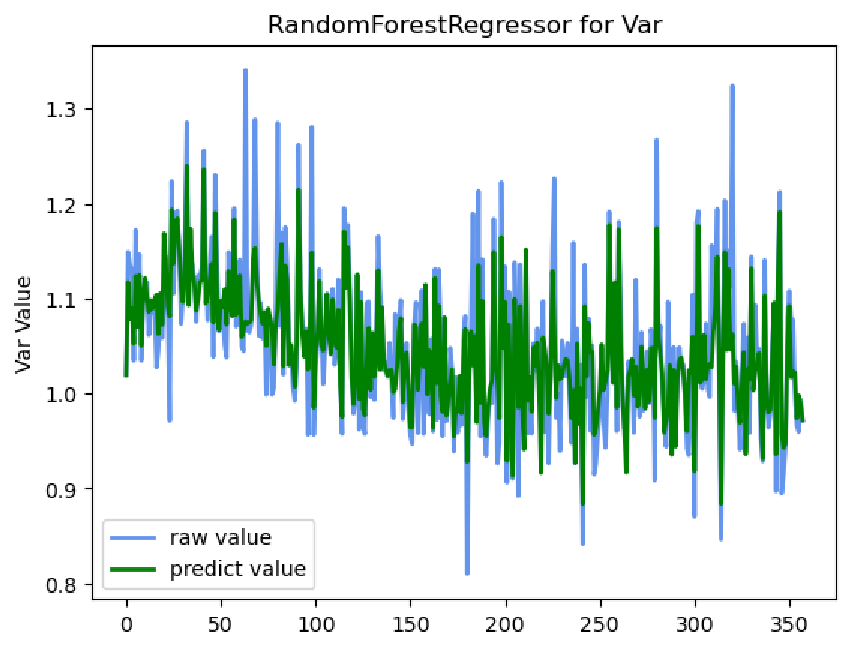
\includegraphics[scale=0.5]{y}   %以pic.jpg的0.5倍大小输出
\end{minipage}
}
\caption{} %  %大图名称
\label{fig:1}  %图片引用标记
\end{figure}


left one: For the return of the training set correlation coefficient ($R^2$) : 0.905 

\hspace*{1.8cm}For the test set of regression correlation coefficient ($R^2$) : 0.398

right one: For the return of the training set correlation coefficient ($R^2$) : 0.908

\hspace*{1.8cm}For the test set of regression correlation coefficient ($R^2$) : 0.357

\subsection{Result} 

\hspace*{0.6cm}A specific example of your prediction for the word EERIE on March 1, 2023. 


The prediction data are $\mu$ : 4.32138891,$\sigma$ : 1.0459

Following the Normal Distribution Law and the formula:

\[f(x)=\frac{1}{\sqrt{2 \pi} \sigma} \exp \left(-\frac{(x-\mu)^2}{2 \sigma^2}\right)\]

we can work out the final proportion below.

[ 0.27080026, 3.37763063, 17.39287034, 36.97648791, 31.08331013, 10.57375257,  0.32514815]


\begin{figure}[h]
\small
\centering
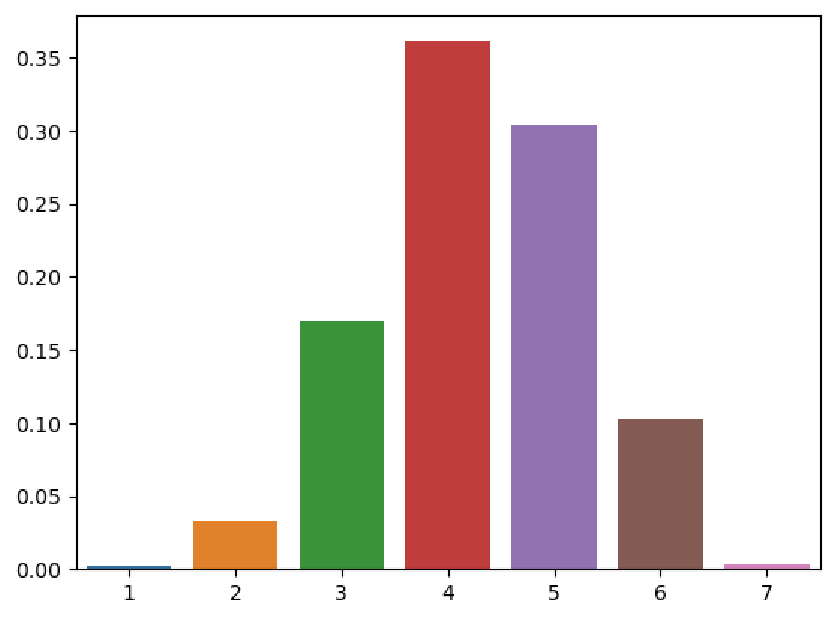
\includegraphics[width=8cm]{yuce}
\caption{Predictions} \label{fig:aa}
\end{figure}

%%%%%%%%%%%%%%%%%%%%%%%%%%%%%%%%%%%%%%%%%%%%%%%%%%%%%%%%%%%%%%%5

\section{Classify Words Model}
\subsection{Problem Analysis}
\begin{itemize}
\item Classification by difficulty: cluster analysis using percentages and included attributes
\item Identify the attributes of a given word associated with each category: use word 
attributes to map the categories with a classification model
\item How hard is the word EERIE?
\item Discuss the accuracy of your classification model that is to say, how well the model performed on the test set
\end{itemize}

Accordingly, the model construction and analysis of the third question can be divided into
four steps:

1. Using percentage and included attributes to do cluster analysis

In this section, we use K-means clustering analysis to cluster the mean value and
standard deviation according to the distance, and fit the probability distribution
histogram for difficulty classification

2. Using word attributes to map classification by classification model

We use the random forest classification model to map the five indicators of word
attributes (EN, TR, GS, YS, CS) and the target formed by the clustering in the first
step, and fit a classifier to facilitate the subsequent word prediction.

3. Put EERIE into a classifier for sorting

We evaluated the word attributes of EERIE, then put them into the trained random
forest model for prediction, and determined the difficulty of the word EERIE.

4. Get a representation of the model's performance on the test set

\begin{figure}[h]
\small
\centering
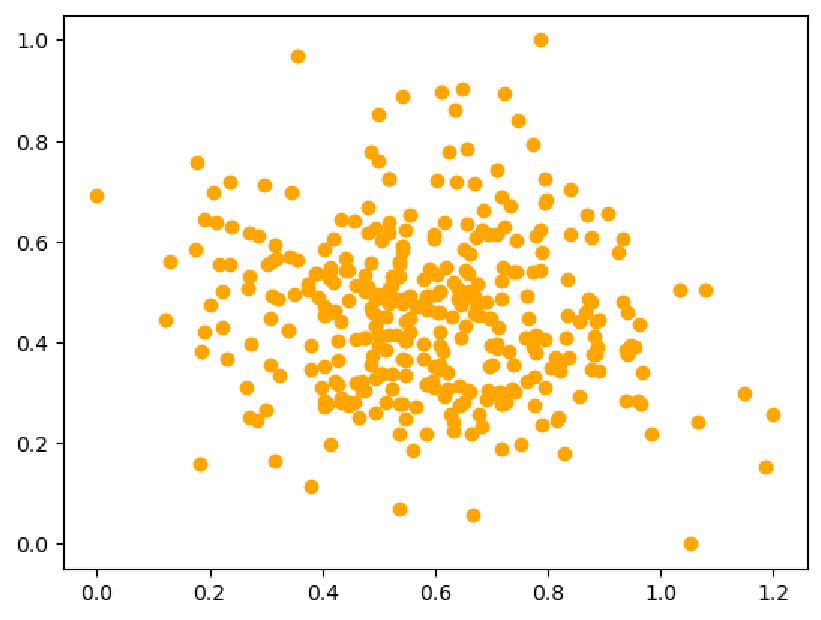
\includegraphics[width=8cm]{sandiantu}
\caption{The scatter plot of mean and standard deviation} \label{fig:aa}
\end{figure}

\subsubsection{Flowchart}

\begin{figure}[h]
\small
\centering
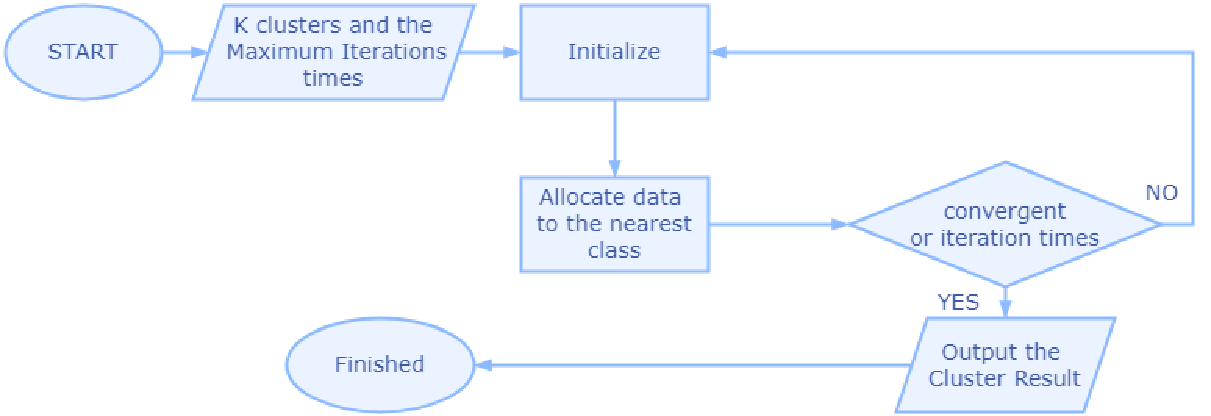
\includegraphics[width=11cm]{Q3}
\caption{Flowchart} \label{fig:aa}
\end{figure}

\subsection{Model Construction}
\subsubsection{Model Principle}

\hspace*{0.6cm}K-means clustering is a common unsupervised learning algorithm used to divide a data set into multiple different groups (clusters). The similarity of data points within each
group is high, while the similarity between different groups is low. The optimization goal
of K-means algorithm is to minimize the Sum of distance (SSE, Sum of Squared Errors)
between each data point and the clustering center of the cluster it belongs to. Therefore,
the main steps of k-means clustering include selecting the appropriate K value, initializing
the clustering center, allocating data points to the cluster, calculating the center point of
the cluster, and iterating until convergence is reached.

The principle of random forest classification is the same as that of random forest
regression used in the second question, so I will not repeat it here.

\subsubsection{Model Assumption}

\hspace*{0.6cm}1. Suppose that the difficulty of the word is described only by the percentage
distribution of the number of reports, independent of other factors such as the
percentage of difficult patterns chosen.

2.Suppose that the percentage distribution of the number of reports is close to a
normal distribution, which can be well described by means and standard deviations
alone.

3. Suppose the mean of the distribution of reporting times can better reflect the
difficulty of words than the standard deviation. In K-means analysis, the weight ratio
of mean to standard deviation is 6:5.

4. Suppose noise caused by chance willn't obscure the feature of standard
deviation and mean

\subsubsection{Main Model}
The first step is to construct the clustering model with K-means clustering

1. The data is normalized and the mean is multiplied by 1.2, making the weight ratio of
mean to standard deviation 6:5.

2. Using elbow method and Silhouette Coefficient, the optimal clustering number was
 be 4

\begin{figure}[htbp]
\centering    %居中
\subfigure[] %第一张子图
{\begin{minipage}{8cm}
\centering          %子图居中
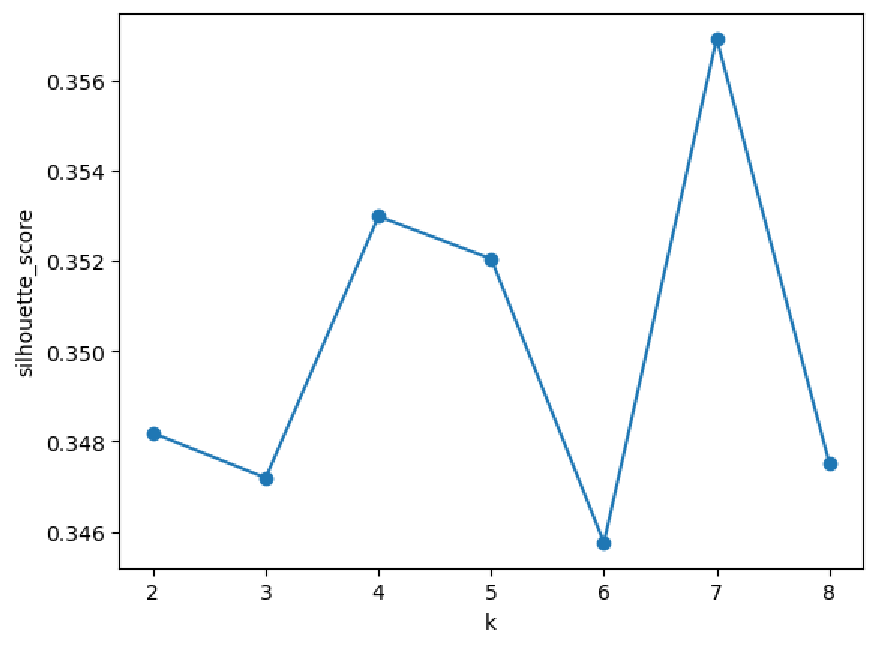
\includegraphics[scale=0.4]{zuo}   %以pic.jpg的0.5倍大小输出
\end{minipage}
}	
\subfigure [] %第二张子图
{\begin{minipage}{8cm}
\centering      %子图居中
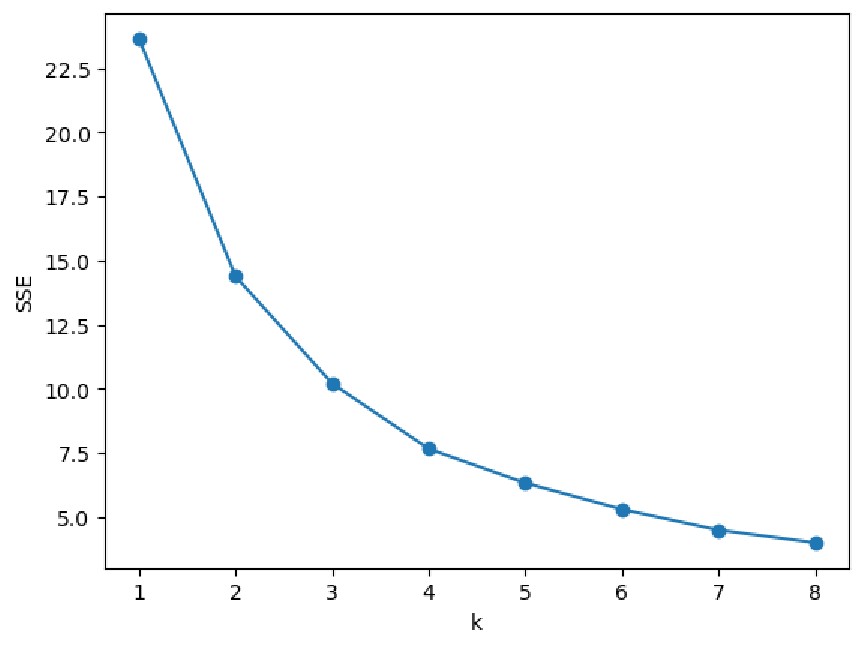
\includegraphics[scale=0.4]{you}   %以pic.jpg的0.5倍大小输出
\end{minipage}
}
\caption{} %  %大图名称
\label{fig:1}  %图片引用标记
\end{figure}

3. Here is the clustering result (the asterisk is the clustering center)

\begin{figure}[h]
\small
\centering
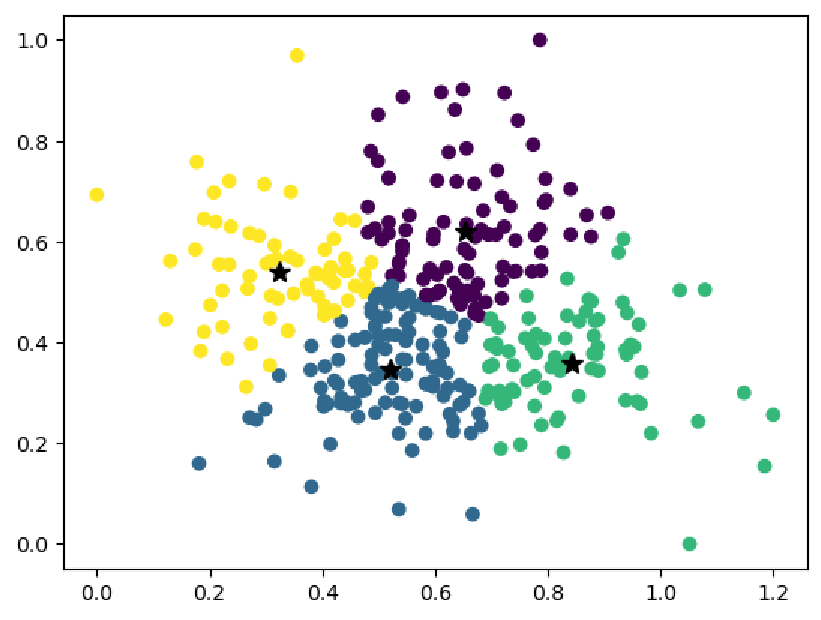
\includegraphics[width=6cm]{julei}
\caption{the clustering result} \label{fig:aa}
\end{figure}

4. The distribution histogram and normal distribution diagram of different difficulty are
summarized

\begin{figure}[htbp]
\centering    %居中
\subfigure[Simple] %第一张子图
{\begin{minipage}{7cm}
\centering          %子图居中
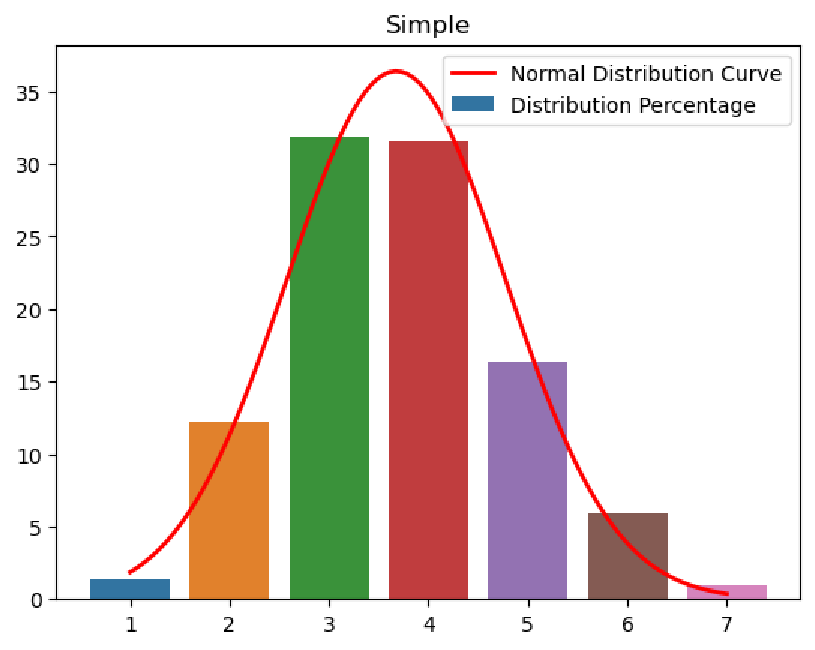
\includegraphics[scale=0.45]{22}   %以pic.jpg的0.5倍大小输出
\end{minipage}
}	
\subfigure [Ordinary] %第二张子图
{\begin{minipage}{7cm}
\centering      %子图居中
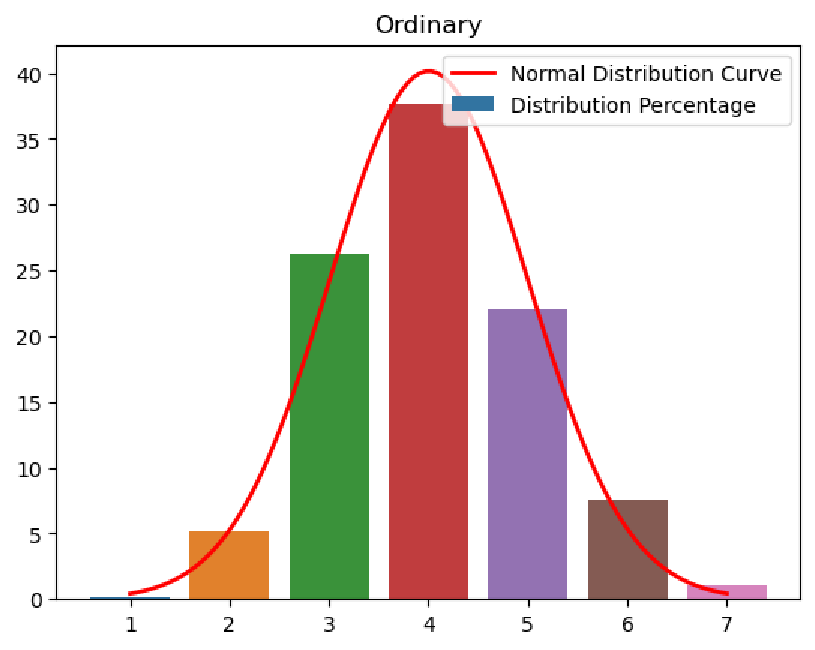
\includegraphics[scale=0.45]{11}   %以pic.jpg的0.5倍大小输出
\end{minipage}
}
\subfigure [Rather Difficult] %第二张子图
{\begin{minipage}{7cm}
\centering      %子图居中
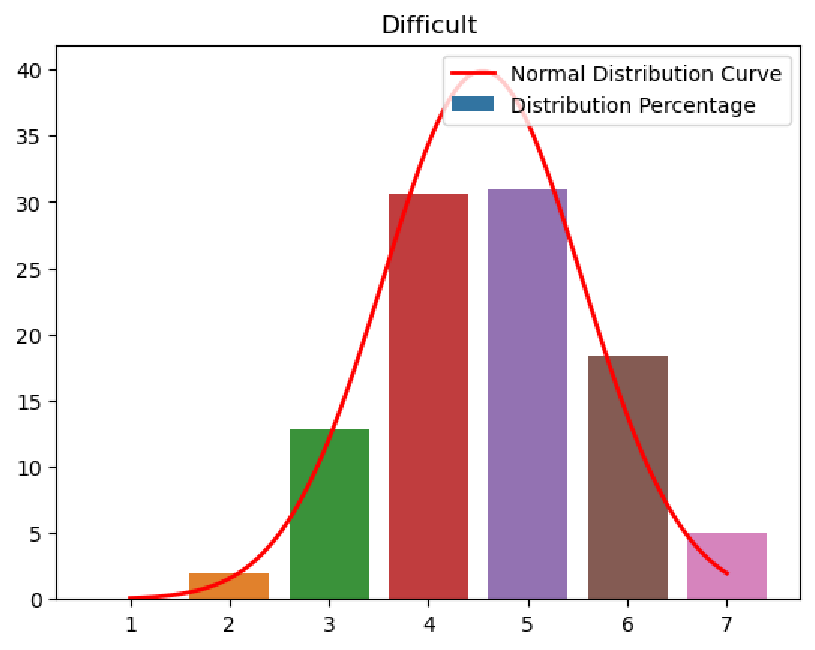
\includegraphics[scale=0.45]{44}   %以pic.jpg的0.5倍大小输出
\end{minipage}
}
\subfigure [Difficult] %第二张子图
{\begin{minipage}{7cm}
\centering      %子图居中
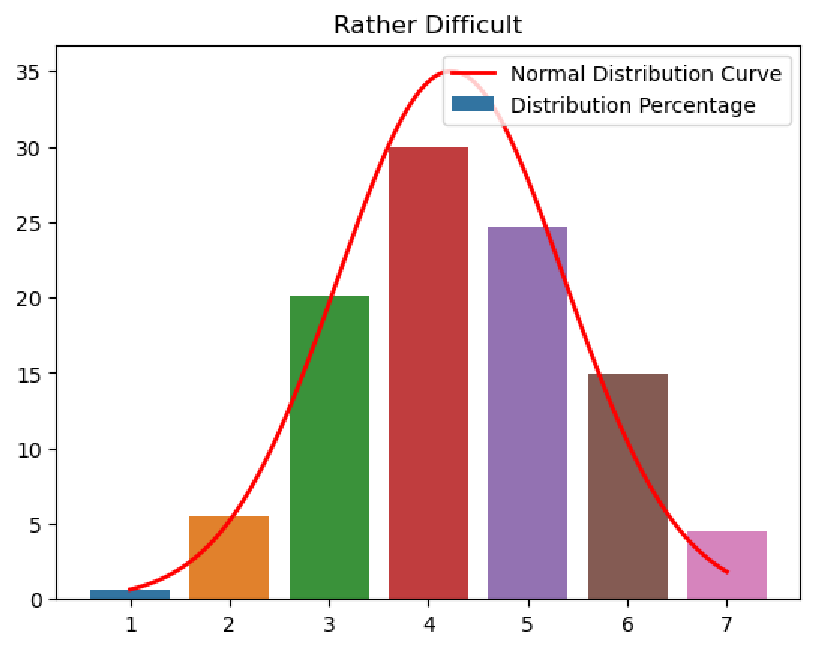
\includegraphics[scale=0.45]{33}   %以pic.jpg的0.5倍大小输出
\end{minipage}
}
\caption{} %  %大图名称
\label{fig:1}  %图片引用标记
\end{figure}


Second, the random forest classification model is no longer used to classify word
features


1. Training random forest classification models

Classified image


\begin{figure}[h]
\small
\centering
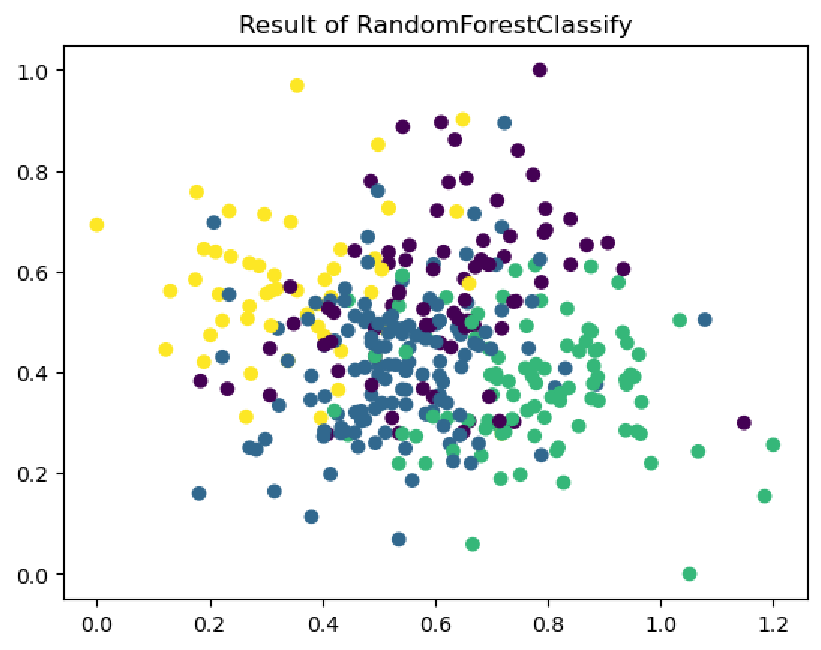
\includegraphics[width=8cm]{aa}
\caption{random forest classification} \label{fig:aa}
\end{figure}

Accuracy for the training set: 0.736

Accuracy for the testing set: 0.523

2. Predict word difficulty: (EERIE)

Predicted classification: (Rather Difficult)

The Classification and Probabilty table shows underneath.

\begin{table}[!htbp]
\begin{center}
\caption{Test Outcome}
\begin{tabular}{cl}
 \toprule
 \multicolumn{1}{m{3cm}}{\centering Classification}
 &\multicolumn{1}{m{4cm}}{\centering Probability(\%)}\\
 \midrule
Simple &   \hspace*{32.2} 9.54 \\
  Ordinary & \hspace*{32.2}   14.09 \\
  Rather difficult & \hspace*{32.2}   13.63 \\
  difficult & \hspace*{32.2}   62.73 \\\bottomrule
\end{tabular}\label{tb:notation}
\end{center}
\end{table}

%%%%%%%%%%%%%%%%%%%%%%%%%%%%%%%%%%%%%%%%%%%%%%%%%%%%%%%%%%%%%%%6

\section{interesting features}
\hspace*{0.6cm}According to the problem, we could learn from the fact that the dataset given by this problem was taken from Twitter, but Twitter's data was not comprehensive since  users have the right to choose whether to report their results. Following the rules of Wordle, users have six chances to get the right answer, Otherwise he/she will fail the game. This game was a little bit difficult for most of us. However, after integrating the percentage of each try times in the dataset, we find most of the users completed the game within 5 trials, and only few (2.8\%) failed the game, which is not in line with our tuition, so we take the assumption that users who reported their results are usually those who completed the game and use less chances.

\begin{figure}[h]
\small
\centering
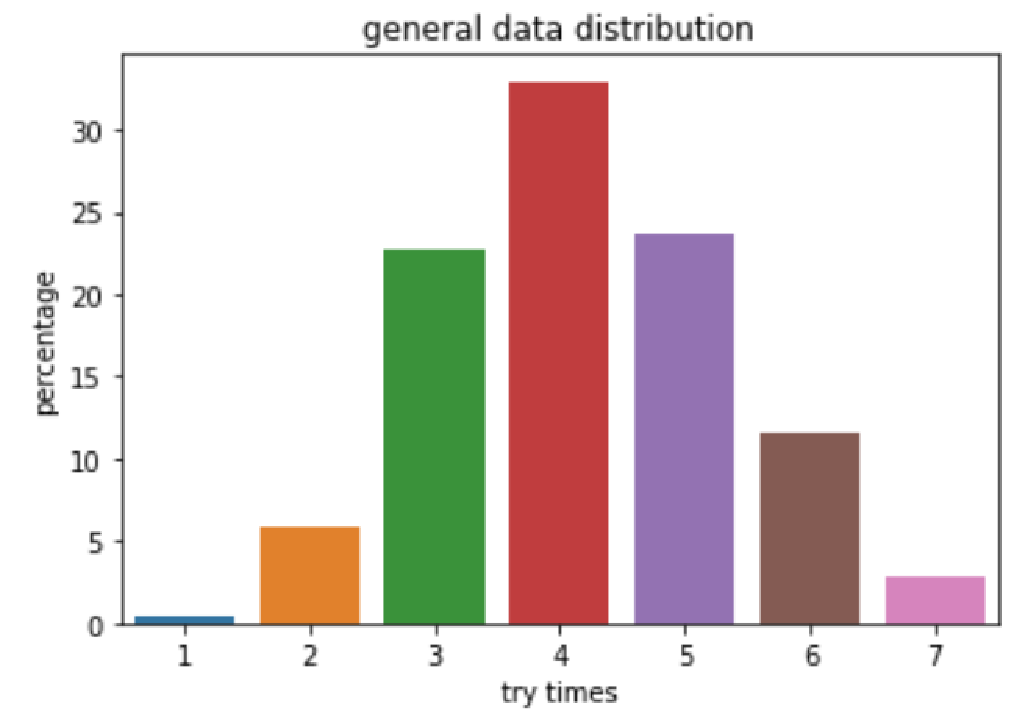
\includegraphics[width=7cm]{barchart}
\caption{The bar chart} \label{fig:aa}
\end{figure}

In order to verify our assumption, we developed a model  to simulate the process of how people guess words  in Wordle.  To simplify this model, we assume people choose words which come to their mind first, which has a high correlation with word frequency in English. So we continuing using the word frequency data taken from wolftram, distributing probabilities to each word according to their frequency, and choose them randomly. the algorithm flow are as follows:

\begin{figure}[h]
\small
\centering
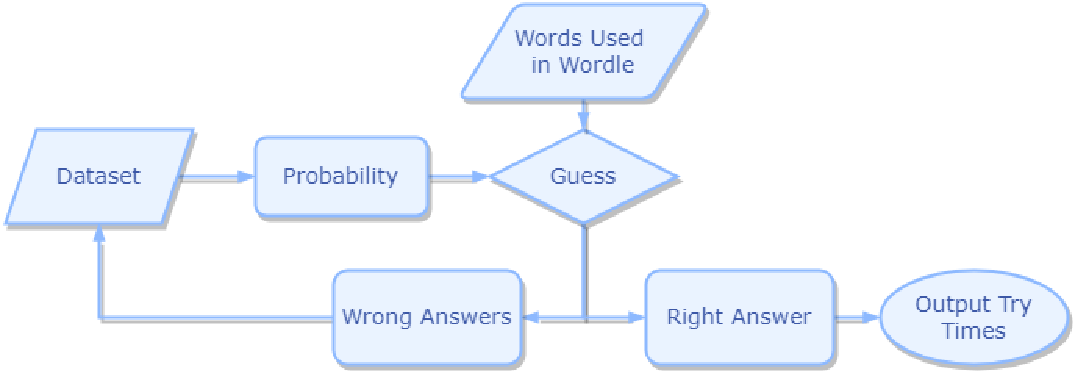
\includegraphics[width=10cm]{Q4}
\caption{The Algorithm Flow} \label{fig:aa}
\end{figure}

We ran each word 20 times to find the average expectation, compared it with the expectation of the known words of the topic, and made a correlation analysis with
hypothesis testing, as shown in the following figure.

\begin{figure}[h]
\small
\centering
\includegraphics[width=8cm]{predictafter}
\caption{The Prediction Result} \label{fig:aa}
\end{figure}

We calculated each word for 20 times, getting their average try time and compare it with the true average try time, seen from the line chart , the predict data was much higher than real data. and the Mean expected difference of these (359 words) was 6.925 (11.046-4.121),which was related to our assumption.

then we need to test the correctness of our algorithm model. we calculated Pearson correlation coefficient, and did hypothesis testing of these 2 data the result of which are as follow:


\begin{longtable}{ p{14em} p{4em} p{4em} }
\caption{Relevance}
\label{tb:longtable}\\
\toprule
 & test & predict \\
\midrule
Pearson Relevence & .533** & \centering 1\\
\midrule
Sig. two-sided hypothesis &  .000 & \\
\bottomrule
\end{longtable}


Since p=0.000<0.01, we are 99\% sure that these 2 data have significant correlation, and the Pearson correlation coefficient is 0.53. We can conclude our model is useful and correct to some extent.

To make further analysis, we integrated all predicted data and real data, getting its distribution and drew its histogram. As can be seen from the image, users who report their data are only the tip of the iceberg of the whole data. Behind the displayed data set, there are a large number of users who fail to guess the word successfully. Most users who share their data on Twitter had figure out the puzzle and had good game scores.


\begin{figure}[h]
\small
\centering
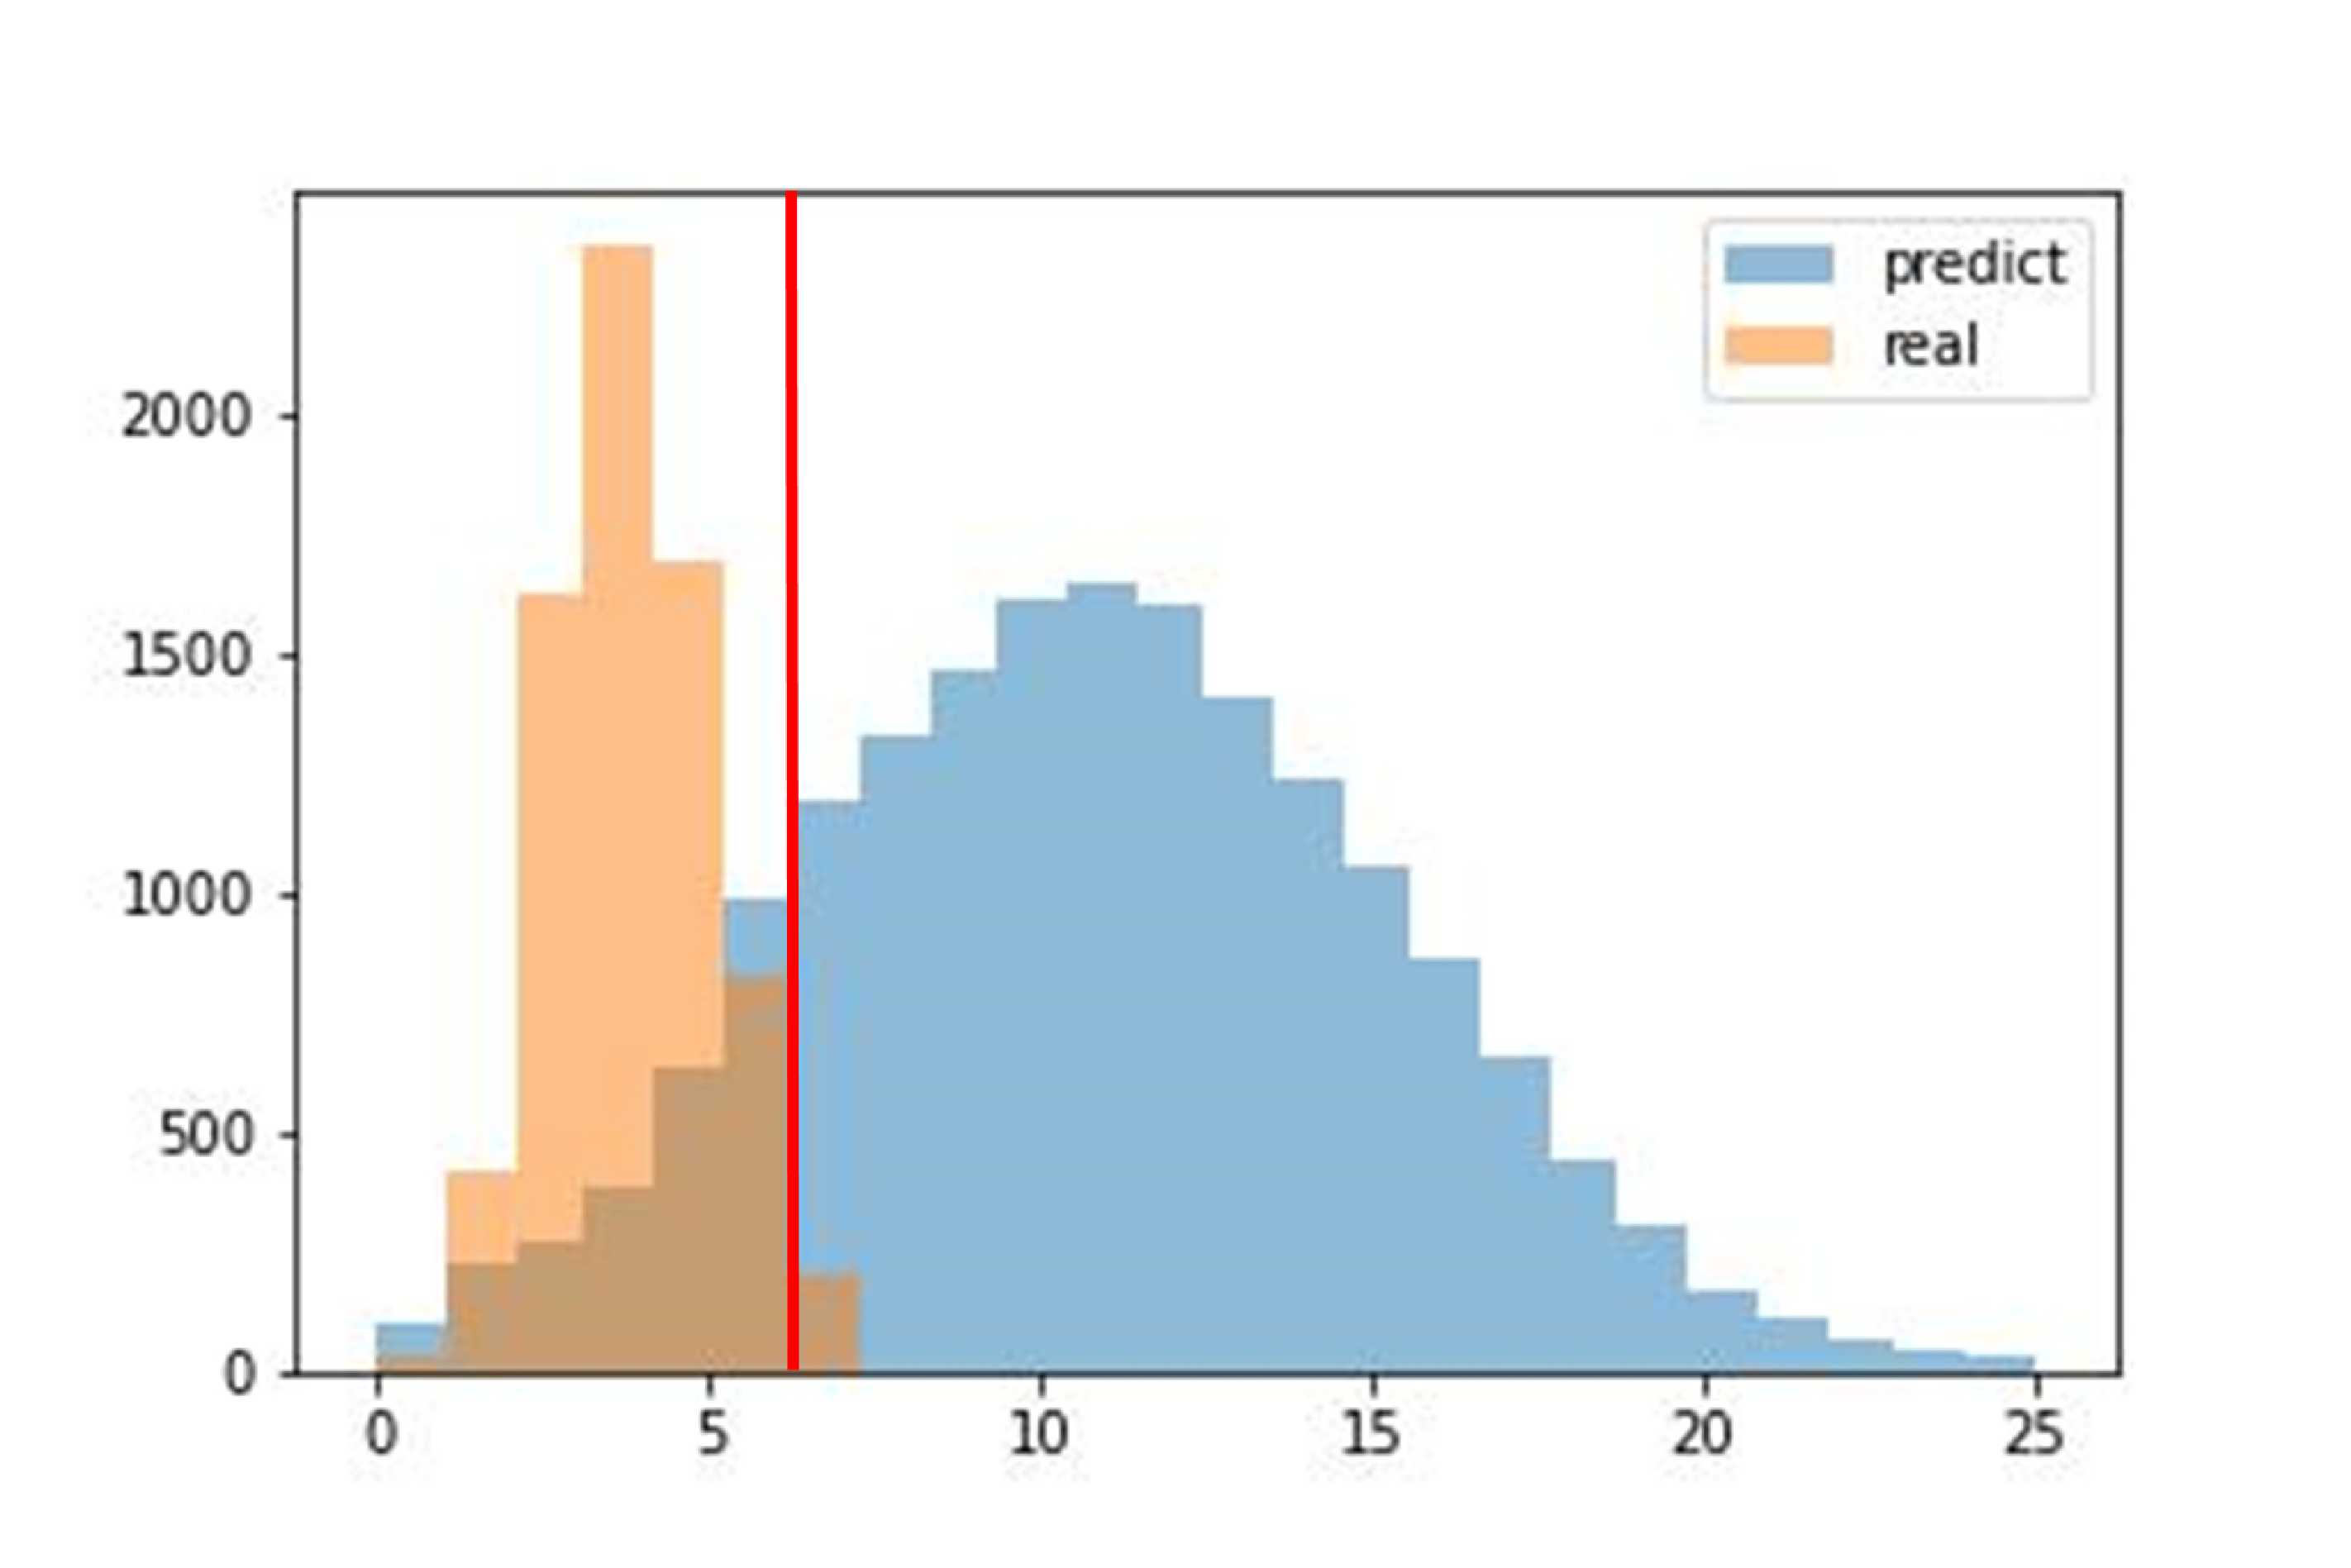
\includegraphics[width=8cm]{mountain}
\caption{Data Mountain and its Knap} \label{fig:aa}
\end{figure}

Based on this model, we try to figure out in what  kind of situation would users like to report their grades: we divide real value by predict value and rescaling it, and draw its line chart

\begin{figure}[h]
\small
\centering
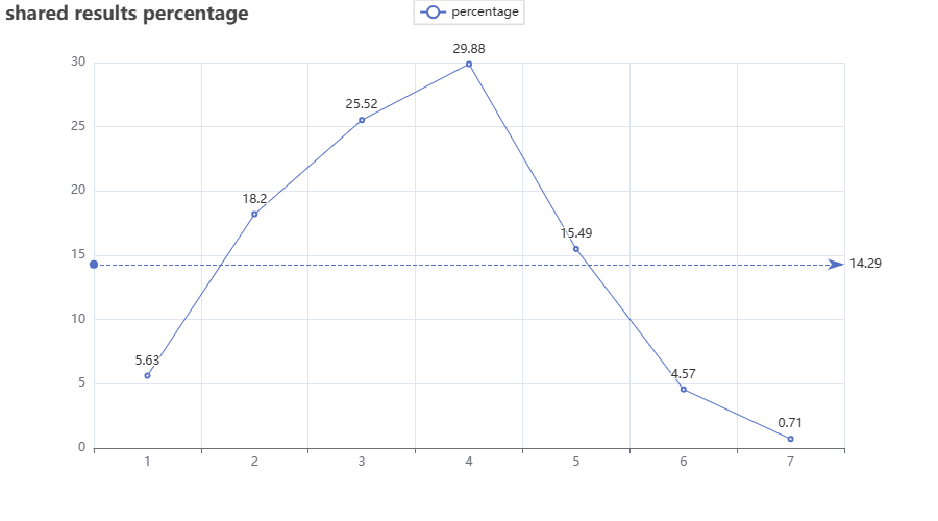
\includegraphics[width=8cm]{linechart}
\caption{The Line Chart} \label{fig:aa}
\end{figure}

Within the allowable range of errors, we find that, unlike the expected results, the proportion of sharing data does not show a monotonically decreasing trend, but first increases and then decreases, and reaches a peak at x=4. Although generally speaking players with better results are more likely to post their grades, the percentage declines when the results are too good (the number of attempts is close to one). We reasoned that such groups guessed words based more on probability than on the amount of information in the question. Rapid success does not make users feel the fun of the game, while users in the interval of 3 to 5 guess data more rely on the information of ideas and topics constantly updated. The stronger the sense of achievement brought to users by guessing words in this interval, it is in line with the inference and expectation of psychology.


















%%%%%%%%%%%%%%%%%%%%%%%%%%%%%%%%%%%%%%%%%%%%%%%%%%%%%%%%%%%%%%%7
\section{Strengths and weaknesses}

\subsection{Strengths}

\hspace*{0.6cm} 1. In problem 1’s number prediction, we use ARIMA time series analysis, and use random forest, the data in February,1,2023 to test its correctness, which verify the robustness of our model

 2. In problem 4, we generate a algorithm that simulate people’s word-guessing process, which predict the true data hind behind the data showed by Twitter, thus we can get some results related to psychology.

\subsection{Weaknesses}
 \hspace*{0.6cm}1. in problem 2, we use normal distribution curve to fit the data, although the percentage predicted at the center is good, the predicted data in x=1 & x=7 or more is not quite precisely.

 2. we use K-means method in problem 3, however, seen from the scatterplot, the data is not quite suitable to do K-means cluster, thus the model may not be robust.















%%%%%%%%%%%%%%%%%%%%%%%%%%%%%%%%%%%%%%%%%%%%%%%%%%%%%%%%%%%%%%%8

\begin{thebibliography}{99}
\bibitem{1} Morning Consult. (2022, January 20). The top 10 mobile games in the US: January 2022. 

\url{https://morningconsult.com/form/top-mobile-games-us-january-2022/}
\bibitem{2}“Wordle Stats.” Twitter, January 1, 2022.
\bibitem{3} OnePoll. (2022). The Wordle survey. https://www.onepoll.us/the-wordle-survey/
\bibitem{4} Oxford English Dictionary. (2022). Entry. In Oxford English Dictionary Online. Retrieved February 20, 2023, from \url{https://www.oed.com/}

\bibitem{5} B. J. Anderson and J. G. Meyer, “Finding the optimal human strategy for wordle using maximum correct letter probabilities and reinforcement learning,” arXiv preprint arXiv:2202.00557, 2022
\bibitem{6}Schriefers, H., & Teruel, E. (2000). The influence of morphological regularities on the processing of compounds: Evidence from event-related potentials. Brain and Language, 72(3), 271-287.
\end{thebibliography}
%%%%%%%%%%%%%%%%%%%%%%%%%%%%%%%%%%%%%%%%%%%%%%%%%%%%%%%%%%%%%%%9
\newpage

\begin{letter}{Dear, Mr. Alpha Chiang}

\hspace*{0.6cm}Thank you for providing us with the data. During four days of work, we created several models and gathered data that may assist you and your company develop Wordle plans. Here are some specifics.

\hspace*{0.6cm}First, we developed a model (ARIMA (4,1,2)) to forecast time series, which will aid you in determining how many people will play games in the future. Using the Random Forest approach and actual data from February 1,2023, this model was tested for robustness. Although Wordle was previously a well-known game and a great hit in America, time series research revealed that active game users progressively became steady and then appeared to slightly decline, which may not be good news for your firm and necessitates the adoption of some new techniques.
	
\hspace*{0.6cm}The model above was then refined by taking word qualities into consideration. This approach, known as Random Forest Regression, may be used to forecast the related percentages of each try with particular dates and words. To display aspects that might affect the percentage distribution, we created a number of features ourselves (word entropy, combination of letters, incidence of single letters, letter location, etc.). As it is more particular, this model was not as reliable as the first one, but it still has a high value for you to make judgments in the future, such choosing which letter to be the response.
	
\hspace*{0.6cm}Using K-means clustering, we divide all of your words into 4 groups (Simple, Ordinary, Difficult, and Quite Difficult), taking into account the aforementioned characteristics (the standards we use are mean & standard derivation). The score of the average user varies depending on the class. The classification of words and a rudimentary understanding of psychology (such as the Cwithfish Effect and Transfinite Effect) might be used to create a technique for giving words from various classes on a recurring basis to better thrill our consumers.
	
\hspace*{0.6cm}Lastly, by factoring in word frequency and probability, we create a model to mimic how humans estimate words. Our model revealed that users who post their grades on Twitter make up a small portion of all users that participate in the game (as can be seen from our essay), and they all have the trait of being mostly game winners. They may become passionate about sharing their results after winning games, which is an excellent kind of promotion. So, raising the maximum attempt times could encourage more users.

\hspace*{0.6cm}That is basically all the work we do, and we all want to see Wordle improve in the future. We hope that our methodology will assist you and your company in creating stronger Wordle plans.
	 
\vspace{\parskip}

\\
\\
Sincerely,

yours 2301434

\end{letter}
\end{document}
